\documentclass[tikz,border=12pt]{standalone}
\usepackage{amsmath}
\usetikzlibrary{arrows.meta}

\begin{document}
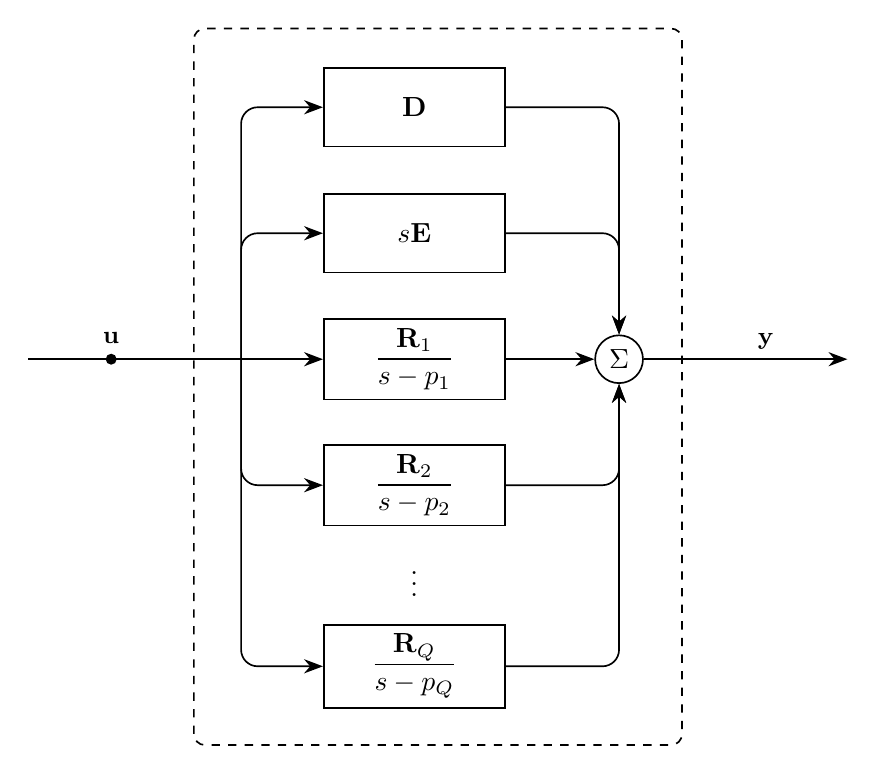
\begin{tikzpicture}[
    >={Stealth[length=2.4mm]},
    line/.style   = {semithick, rounded corners=6pt},
    block/.style  = {draw, semithick, fill=white,
                     minimum height=1cm, minimum width=2.3cm},
    sum/.style    = {draw, semithick, fill=white, circle, inner sep=2.6pt},
    signal/.style = {circle, fill, inner sep=1.4pt, label distance=3pt},
    sig/.style    = {font=\small}
]

% Parallel branches
\node[block] (D) at (0, 3.2) {$\mathbf{D}$};
\node[block] (E) at (0, 1.6) {$s\mathbf{E}$};
\foreach \q/\y in {1/0, 2/-1.6, Q/-3.9}
    \node[block] (R\q) at (0, \y) {$\dfrac{\mathbf{R}_{\q}}{s - p_{\q}}$};
\node at (0, -2.75) {$\vdots$};

% Fan-out from a single internal point
\coordinate (split) at (-2.2, 0);
\draw[line] (-4.9, 0) -- (split);
\draw[->, line] (split) -- (R1.west);
\foreach \b in {D, E, R2, RQ}
    \draw[->, line] (split) |- (\b.west);

% Fan-in to summation
\node[sum] (S) at (2.6, 0) {$\Sigma$};
\draw[->, line] (R1.east) -- (S);
\foreach \b/\a in {D/north, E/north, R2/south, RQ/south}
    \draw[->, line] (\b.east) -| (S.\a);
\draw[->, line] (S.east) -- (5.5, 0) node[sig, pos=0.6, above] {$\mathbf{y}$};

% Signal node: u external
\node[signal, label={[sig]above:$\mathbf{u}$}] at (-3.85, 0) {};

% Model enclosure
\draw[dashed, semithick, rounded corners=4pt] (-2.8, -4.9) rectangle (3.4, 4.2);

\end{tikzpicture}
\end{document}
